\documentclass[12pt,a4paper]{article}
\usepackage{ugmath}
\usepackage{float}
\usepackage{placeins}
\usepackage [spanish]{babel}
\usepackage[labelfont=bf,labelsep=space]{caption}
\newcommand{\paren}[1]{\left( #1 \right)}
\newcommand{\alumno}{Ricardo León Martínez}
\newcommand{\materia}{Calculo Diferencial e Integral II}
\newcommand{\profesor}{Fernando Nuñez Medina}
\newcommand{\tarea}{Tarea 7}
\newcommand{\fecha}{20/3/2026}

\begin{document}
    \begin{center}
    {\large\textbf{UNIVERSIDAD DE GUANAJUATO}}\\[0.3cm]
    {\normalsize\textbf{DIVISIÓN DE CIENCIAS NATURALES Y EXACTAS}}\\
    {\normalsize\textbf{CAMPUS GUANAJUATO}}\\[1cm]

    {\Large\textbf{\tarea\ (\materia)}}\\[1cm]
    \end{center}

    \textbf{Nombre:} \alumno \hfill 
    \textbf{Fecha:} \fecha \hfill 
    \textbf{Calificación:} \rule{3cm}{0.4pt} \\[0.3cm]

    \begin{mdframed}[style=mdbluebox,frametitle={Ejercicio 1}]
        Muestra que el área de la superficie de la esfera con centro en el origen y radio $r$ es
        $4\pi r^{2}$.
    \end{mdframed}

    \begin{proof}
        Consideremos la semicircunferencia superior de radio $r$ centrada en el origen,
        cuya ecuación está dada por
        \begin{equation*}
            y=\sqrt{r^{2}-x^{2}}
        \end{equation*}
        Al rotar esta curva alrededor del eje $x$ se genera la superficie de una esfera de radio $r$.
        El área de una superficie de revolución obtenida al rotar una función $y=f(x)$ alrededor del
        eje $x$ está dada por
        \begin{equation*}
            S=2\pi\int_{a}^{b}f(x)\sqrt{1+(f^{\prime}(x))^{2}}dx.
        \end{equation*}
        Aplicando esto a $f(x)=\sqrt{r^{2}-x^{2}}$ en el intervalo $[-r,r]$ obtenemos
        \begin{equation*}
            S=2\pi\int_{-r}^{r}\sqrt{r^{2}-x^{2}}\sqrt{1+(f^{\prime}(x))^{2}}dx.
        \end{equation*}
        Derivamos $f(x)$ por tanto
        \begin{equation*}
            f^{\prime}(x)=\frac{-x}{\sqrt{r^{2}-x^{2}}}
        \end{equation*}
        y entonces
        \begin{equation*}
            1+(f^{\prime}(x))^{2}=1+\frac{x^{2}}{r^{2}-x^{2}}=\frac{r^{2}}{r^{2}-x^{2}}.
        \end{equation*}
        En consecuencia
        \begin{equation*}
            \sqrt{1+(f^{\prime}(x))^{2}}=\frac{r}{\sqrt{r^{2}-x^{2}}}.
        \end{equation*}
        Sustituyendo en la Integral
        \begin{align*}
            S&=2\pi\int_{-r}^{r}\sqrt{r^{2}-x^{2}}\frac{r}{\sqrt{r^{2}-x^{2}}}dx\\
            &=2\pi r\int_{-r}^{r}dx\\
            &=[2\pi rx]_{-r}^{r}\\
            &=(2\pi r^{2})-(-2\pi r^{2})\\
            &=4\pi r^{2}.
        \end{align*}
        Así, el area de una esfera de radio $r$ es $4\pi r^{2}$.
    \end{proof}

    \begin{mdframed}[style=mdbluebox,frametitle={Ejercicio 2}]
        Utiliza la circunferencia trigonométrica para calcular el valor de las fucniones trigonométricas
        del angulo $\theta$ de cada uno de los incisos siguientes (haz un dibujo).
        \begin{multicols}{2}
            \begin{enumerate}
                \item[(a)]  $\theta=\pi/6.$
                \item[(b)]  $\theta=\pi/3.$
            \end{enumerate}
        \end{multicols}
        \textbf{Sugerencia:} Mediante un triángulo rectángulo muestra que $\sin(\pi/6)=\cos(\pi/3)$ y
        $\cos(\pi/6)=\sin(\pi/3)$; usa lo anterior y las identidades trigonometricas
        \begin{equation*}
            \sin(x+y)=\sin(x)\cos(y)+\sin(y)\cos(x)
        \end{equation*}
        y
        \begin{equation*}
            \cos(x+y)=\cos(x)\cos(y)-\sin(x)\sin(y)
        \end{equation*}
        para mostrar que $\sin(\pi/6)=\frac{1}{2}=\cos(\pi/3)$ y $\cos(\pi/6)=\sqrt{3}/2=\sin(\pi/3)$.
    \end{mdframed}

    \begin{solucion}
        \begin{enumerate}
            \item[(a)] $\theta=\pi/6$\\
            En un triangulo rectangulo $30^{\circ}-60^{\circ}-90^{\circ}$ se tiene
            \begin{equation*}
                \sin(\frac{\pi}{6})=\frac{1}{2},\qquad \cos(\frac{\pi}{6})=\frac{\sqrt{3}}{2}.
            \end{equation*}
            Además, como
            \begin{equation*}
                \frac{\pi}{6}+\frac{\pi}{3}=\frac{\pi}{2},
            \end{equation*}
            usando la proposición 31 se sigue que
            \begin{equation*}
                \sin(\frac{\pi}{2})=\sin(\frac{\pi}{6})\cos(\frac{\pi}{3})+\sin(\frac{\pi}{3})\cos(\frac{\pi}{6})
            \end{equation*}
            Como $\sin(\pi/2)=1$ y usando que
            \begin{equation*}
                \sin(\frac{\pi}{6})=\cos(\frac{\pi}{3}), \quad \cos(\frac{\pi}{6})=\sin(\frac{\pi}{3})
            \end{equation*}
            se tiene que
            \begin{equation*}
                \sin(\frac{\pi}{6})=\frac{1}{2},\qquad \cos(\frac{\pi}{6})=\frac{\sqrt{3}}{2}.
            \end{equation*}
            De aqui tenemos que
            \begin{equation*}
                \tan(\frac{\pi}{6})=\frac{1}{\sqrt{3}},\qquad \csc(\frac{\pi}{6})=2\qquad\sec(\frac{\pi}{6})=\frac{2}{\sqrt{3}}\qquad\cot(\frac{\pi}{6})=\sqrt{3}.
            \end{equation*}
            \begin{center}
                
\includegraphics[width=0.35\textwidth]{a.pdf}
            \end{center}
            \item[(b)] $\theta=\pi/3$\\
            Usando las relaciones del inciso anterior
            \begin{equation*}
                \sin(\frac{\pi}{3})=\cos(\frac{\pi}{6}),\qquad\cos(\frac{\pi}{3})=\sin(\frac{\pi}{6})
            \end{equation*}
            Por lo tanto
            \begin{equation*}
                \sin(\frac{\pi}{3})=\frac{\sqrt{3}}{2},\qquad\cos(\frac{\pi}{3})=\frac{1}{2}.
            \end{equation*}
            Concluyendo que
            \begin{equation*}
                \tan(\frac{\pi}{3})=\sqrt{3},\qquad \csc(\frac{\pi}{3})=\frac{2}{\sqrt{3}},\qquad\sec(\frac{\pi}{3})=2,\qquad\cot(\frac{\pi}{3})=\frac{1}{\sqrt{3}}
            \end{equation*}
            \begin{center}
                
\includegraphics[width=0.35\textwidth]{b.pdf}
            \end{center}
        \end{enumerate}
    \end{solucion}

    \begin{mdframed}[style=mdbluebox,frametitle={Ejercicio 3}]
        Prueba el corolario 2
    \end{mdframed}

    \begin{proof}
        \begin{enumerate}
            \item[(a)] $\sin(2x)=2\sin(x)\cos(x)$.\\
            Por la proposición 31 se tiene
            \begin{equation*}
                \sin(x+y)=\sin(x)\cos(y)+\sin(y)\cos(x).
            \end{equation*}
            Tomando $x=y$ en la identidad anterior obtenemos
            \begin{align*}
                \sin(x+x)&=\sin(x)\cos(x)+\sin(x)\cos(x)\\
                &=2\sin(x)\cos(x).
            \end{align*}
            Por lo tanto, $\sin(2x)=2\sin(x)\cos(x)$.
            \item[(b)] $\cos(2x)=\cos^{2}(x)-\sin^{2}(x)$.\\
            Por la proposición 31 se tiene
            \begin{equation*}
                \cos(x+y)=\cos(x)\cos(y)-\sin(x)\sin(y).
            \end{equation*}
            Tomando $x=y$ en la identidad anterior obtenemos
            \begin{align*}
                \cos(x+x)&=\cos(x)\cos(x)-\sin(x)\sin(x)\\
                &=\cos^{2}(x)-\sin^{2}(x)
            \end{align*}
            Por lo tanto, $\cos(2x)=\cos^{2}(x)-\sin^{2}(x)$.
            \item[(c)] $\tan(2x)=\frac{2\tan(x)}{1-\tan^{2}(x)}$.\\
            Por el corolario 1 se tiene
            \begin{equation*}
                \tan(x+y)=\frac{\tan(x)+\tan(y)}{1-\tan(x)\tan(y)}.
            \end{equation*}
            Tomando $x=y$ en la identidad anterior obtenemos
            \begin{align*}
                \tan(x+x)&=\frac{\tan(x)+\tan(x)}{1-\tan(x)\tan(x)}\\
                &=\frac{2\tan(x)}{1-\tan^{2}(x)}.
            \end{align*}
            Por lo tanto $\tan(2x)=\frac{2\tan(x)}{1-\tan^{2}(x)}$.
        \end{enumerate}
    \end{proof}

    \begin{mdframed}[style=mdbluebox,frametitle={Ejercicio 4}]
        Prueba el inciso (c) de la proposición 37. \textbf{Sugerencia:} Prueba el
        inciso (c) primero cuando $r$ es un número natural, luego cunado $r$ es un número
        entero y finalmente cuando $r$ es un número racional.
    \end{mdframed}

    \begin{proof}
        Por la propiedad (a) se tiene para $n\in\mathbb{N}$
        \begin{equation*}
            \exp(nx)=(\exp(x))^{n}.
        \end{equation*}
        Ademas para $n\in\mathbb{N}$
        \begin{equation*}
            \exp(-nx)=\frac{1}{\exp(nx)}=(\exp(x))^{-n}.
        \end{equation*}
        Por tanto, la identidad vale para todo $p\in\mathbb{Z}$
        \begin{equation*}
            \exp(px)=(\exp(x))^{p}
        \end{equation*}
        Ahora consideremos $r=\frac{p}{q}$. Observemos que
        \begin{equation*}
            q(rx)=px.
        \end{equation*}
        Aplicando la exponencial
        \begin{equation*}
            \exp(q(rx))=\exp(px)
        \end{equation*}
        Usando la propiedad (a)
        \begin{equation*}
            (\exp(rx))^{q}=(\exp(x))^{p}
        \end{equation*}
        Tomando la raiz $q$-ésima en ambos lados
        \begin{equation*}
            \exp(rx)=(\exp(x))^{\frac{p}{q}}
        \end{equation*}
        Así,
        \begin{equation*}
            \exp(rx)=(\exp(x))^{r}
        \end{equation*}
    \end{proof}

    \begin{mdframed}[style=mdbluebox,frametitle={Ejercicio 5}]
        \textbf{(La función $x^{p}$ (continuación))} Sea $0\lt p\lt\infty$ y consideremos
        a la función
        \begin{equation*}
            f(x)=x^{p},0\lt x\lt\infty.
        \end{equation*}
        \begin{enumerate}
            \item[(a)] Muestra que $f$ es creciente.
            \item[(b)] Muestra que $f$ es cóncava hacia abajo si $0\lt p\lt1$ y cóncava
            hacia arriba si $1\lt p\lt\infty$.
            \item[(c)] Muestra que
            \begin{equation*}
                \lim_{x\to0^{+}}x^{p}=0\text{ y }\lim_{x\to\infty}x^{p}=\infty.
            \end{equation*}
            \item[(d)] Dibuja las gráficas de las funciones $x^{2},x^{\frac{1}{2}}$ y $x^{\sqrt{2}}$.
            \item[(e)] Dibuja las gráficas de las funciones $x^{3},x^{\frac{1}{3}}$ y $x^{\sqrt{3}}$. 
        \end{enumerate}
    \end{mdframed}

    \vspace{2.5cm}

    \begin{solucion}
        \begin{enumerate}
            \item[(a)] Muestra que $f$ es creciente.\\
            Derivando
            \begin{equation*}
                f^{\prime}(x)=px^{p-1}.
            \end{equation*}
            Como $x\gt0$ y $p\gt0$, se tiene
            \begin{equation*}
                f^{\prime}(x)\gt0\text{ para todo }x\gt0
            \end{equation*}
            Por lo tanto $f$ es creciente en $(0,\infty)$.
            \item[(b)] Muestra que $f$ es cóncava hacia abajo si $0\lt p\lt1$ y cóncava
            hacia arriba si $1\lt p\lt\infty$.\\
            Calculamos las dos primeras derivadas. Primera derivada
            \begin{equation*}
                f^{\prime}(x)=px^{p-1}
            \end{equation*}
            Segunda derivada
            \begin{equation*}
                f^{\prime\prime}(x)=p(p-1)x^{p-2}.
            \end{equation*}
            Observemos que para todo $x\gt0$
            \begin{equation*}
                x^{p-2}\gt0.
            \end{equation*}
            Por tanto, el signo de $f^{\prime\prime}(x)$ unicamente depende de $p(p-1)$.
            Si $0\lt p\lt1$. Entonces
            \begin{equation*}
                p\gt0,\quad p-1\lt0\implies p(p-1)\lt0.
            \end{equation*}
            Por lo tanto
            \begin{equation*}
                f^{\prime\prime}(x)\lt0\quad\forall x\gt0.
            \end{equation*}
            Así, $f$ es concava hacia abajo en $(0,\infty)$. Si $1\lt p\lt\infty$.
            Entonces
            \begin{equation*}
                p\gt0,\quad p-1\gt0\implies p(p-1)\gt0.
            \end{equation*}
            Por lo tanto
            \begin{equation*}
                f^{\prime\prime}(x)\gt0\quad\forall x\gt0
            \end{equation*}
            $f$ es concava hacia arriba $(0,\infty)$.
            \item[(c)] Muestra los limites.\\
            Veamos que
            \begin{equation*}
                x^{p}=\exp(p\ln(x))
            \end{equation*}
            Sabemos que
            \begin{equation*}
                \lim_{x\to0^{+}}\ln(x)=-\infty.
            \end{equation*}
            Entonces
            \begin{equation*}
                \lim_{x\to0^{+}}p\ln(x)=-\infty,
            \end{equation*}
            y por continuidad de la exponencial
            \begin{equation*}
                \lim_{x\to0^{+}}x^{p}=\lim_{x\to0^{+}}\exp(p\ln(x))=\exp(-\infty)=0.
            \end{equation*}
            De nuevo
            \begin{equation*}
                x^{p}=\exp(p\ln(x))
            \end{equation*}
            Como
            \begin{equation*}
                \lim_{x\to \infty}\ln(x)=\infty,
            \end{equation*}
            entonces
            \begin{equation*}
                \lim_{x\to\infty}p\ln(x)=\infty,
            \end{equation*}
            y por continuidad
            \begin{equation*}
                \lim_{x\to\infty}x^{p}=\exp(\infty)=\infty
            \end{equation*}
            \item[(d)] Dibuja las gráficas de las funciones $x^{2},x^{\frac{1}{2}}$ y $x^{\sqrt{2}}$.
            \begin{figure}[ht]
                \centering
                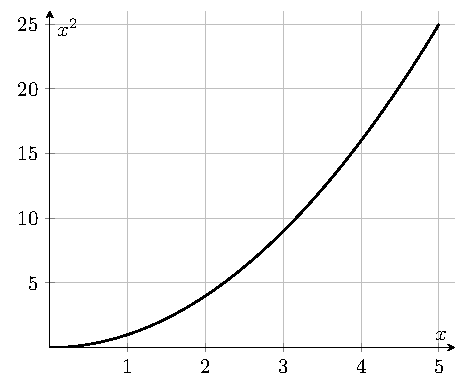
\includegraphics[width=0.32\textwidth]{d-1.pdf}
                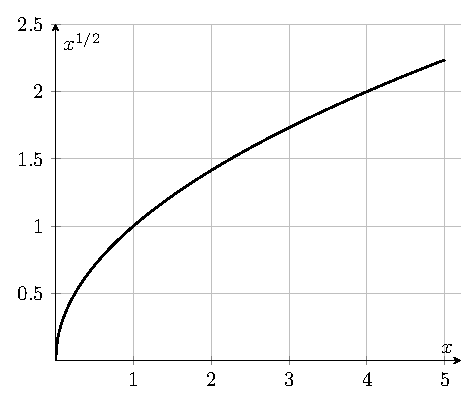
\includegraphics[width=0.32\textwidth]{d-2.pdf}
                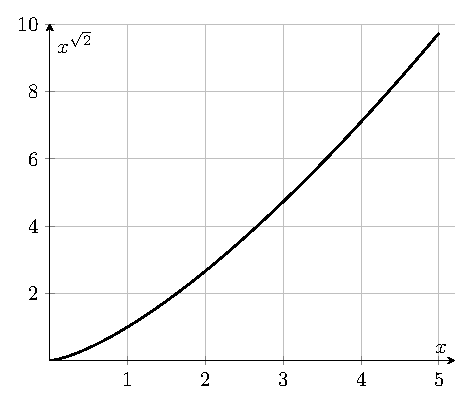
\includegraphics[width=0.32\textwidth]{d-3.pdf}
            \end{figure}
            \item[(e)] Dibuja las gráficas de las funciones $x^{3},x^{\frac{1}{3}}$ y $x^{\sqrt{3}}$.\\
            \begin{figure}[ht]
                \centering
                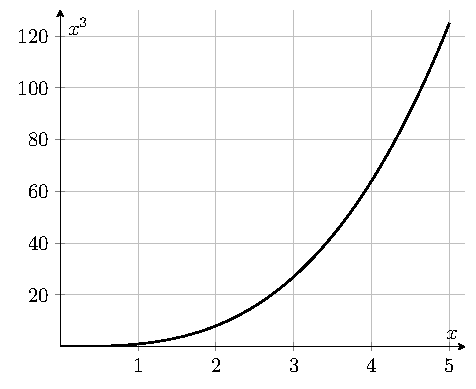
\includegraphics[width=0.32\textwidth]{e-1.pdf}
                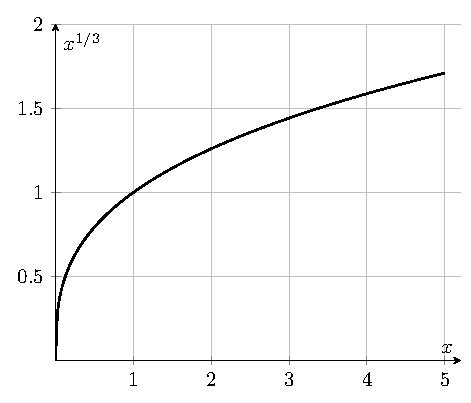
\includegraphics[width=0.32\textwidth]{e-2.pdf}
                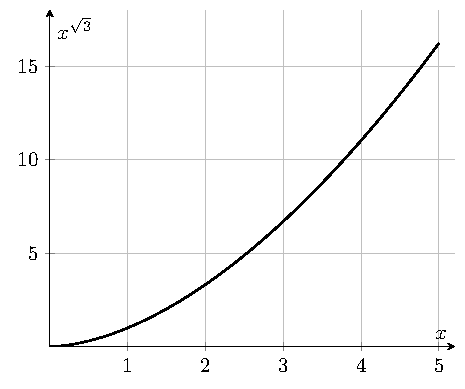
\includegraphics[width=0.32\textwidth]{e-3.pdf}
            \end{figure}
        \end{enumerate}
    \end{solucion}

    \begin{mdframed}[style=mdbluebox,frametitle={Ejercicio 6}]
        Prueba que $a_{n}\to L$ ssi $a_{n}-L\to0$.
    \end{mdframed}

    \begin{proof}
        Supongamos que
        \begin{equation*}
            a_{n}\to L
        \end{equation*}
        Por definicion tenemos que
        \begin{equation*}
            \forall\varepsilon\gt0,\exists N\in\mathbb{N}\text{ tal que }n\geq N\implies\abs{a_{n}-L}\lt\varepsilon
        \end{equation*}
        Pero esta es exactamente
        \begin{equation*}
            \abs{a_{n}-L-0}\lt\epsilon
        \end{equation*}
        Por lo tanto
        \begin{equation*}
            a_{n}-L \to0.
        \end{equation*}
        Supongamos ahora que
        \begin{equation*}
            a_{n}-L\to0
        \end{equation*}
        Entonces, por definición
        \begin{equation*}
            \forall\varepsilon\gt0,\exists N\in\mathbb{N}\text{ tal que }n\geq N\implies\abs{(a_{n}-L)-0}\lt\varepsilon
        \end{equation*}
        Esto equivale a
        \begin{equation*}
            \abs{a_{n}-L}\lt\varepsilon
        \end{equation*}
        Por definición de limite
        \begin{equation*}
            a_{n}\to L.
        \end{equation*}
    \end{proof}

    \begin{mdframed}[style=mdbluebox,frametitle={Ejercicio 7}]
        Calcula los limites siguientes:
        \begin{multicols}{2}
            \begin{enumerate}
                \item[(a)]  $\underset{n\rightarrow\infty}{\lim}\frac{5n^{4}-4n^{2}}{3n^{3}+2n}.$
                \vspace{0.1cm}
                \item[(b)]  $\underset{n\rightarrow\infty}{\lim}\frac{5n^{4}-4n^{2}}{3n^{4}+2n}.$
                \vspace{0.1cm}
                \item[(c)]  $\underset{n\rightarrow\infty}{\lim}\frac{5n^{3}-4n^{2}}{3n^{4}+2n}.$
            \end{enumerate}
        \end{multicols}
    \end{mdframed}

    \begin{solucion}
        \begin{enumerate}
            \item[(a)]  $\underset{n\rightarrow\infty}{\lim}\frac{5n^{4}-4n^{2}}{3n^{3}+2n}.$\\
            Dividimos entre $n^{2}$
            \begin{equation*}
                \lim_{n\to\infty}\frac{5n-\frac{4}{n}}{3+\frac{2}{n^{2}}}
            \end{equation*}
            Al tomar el limite
            \begin{equation*}
                5n\to\infty,\quad\frac{4}{n}\to0,\quad\frac{2}{n^{2}}\to0,
            \end{equation*}
            Por lo tanto
            \begin{equation*}
                \underset{n\rightarrow\infty}{\lim}\frac{5n^{4}-4n^{2}}{3n^{3}+2n}=+\infty
            \end{equation*}
            \item[(b)]  $\underset{n\rightarrow\infty}{\lim}\frac{5n^{4}-4n^{2}}{3n^{4}+2n}.$\\
            Dividimos entre $n^{4}$
            \begin{equation*}
                \lim_{n\to\infty}\frac{5-\frac{4}{n^{2}}}{3+\frac{2}{n^{2}}}
            \end{equation*}
            Pasando al limite
            \begin{equation*}
                \frac{5-0}{3+0}=\frac{5}{3}.
            \end{equation*}
            Así
            \begin{equation*}
                \underset{n\rightarrow\infty}{\lim}\frac{5n^{4}-4n^{2}}{3n^{4}+2n}=\frac{5}{3}
            \end{equation*}
            \item[(c)]  $\underset{n\rightarrow\infty}{\lim}\frac{5n^{3}-4n^{2}}{3n^{4}+2n}.$\\
            Dividimos entre $n^{4}$
            \begin{equation*}
                \lim_{n\to\infty}\frac{\frac{5}{n}-\frac{4}{n^{2}}}{3+\frac{2}{n^{2}}}
            \end{equation*}
            Al tomar el limite
            \begin{equation*}
                \frac{0-0}{3+0}=\frac{5}{3}.
            \end{equation*}
            Así
            \begin{equation*}
                \underset{n\rightarrow\infty}{\lim}\frac{5n^{3}-4n^{2}}{3n^{4}+2n}=0.
            \end{equation*}
        \end{enumerate}
    \end{solucion}

    \begin{mdframed}[style=mdbluebox,frametitle={Ejercicio 8}]
        Prueba que la sucesión
        \begin{equation*}
            \sqrt{2},\sqrt{2\sqrt{2}},\sqrt{2\sqrt{2\sqrt{2}}},\dots
        \end{equation*}
        converge y calcula su límite. \textbf{Sugerencia:} Ten presente que si
        $(a_{n})$ es la sucesión anterior y $a_{n}\to L$, entonces $a_{n+1}=\sqrt{2a_{n}}\to\sqrt{2L}$.
    \end{mdframed}

    \begin{proof}
        Sea la sucesión $a_{n}$ definida por
        \begin{equation*}
            a_{1}=\sqrt{2}\qquad a_{n+1}=\sqrt{2a_{n}},\quad n\in\mathbb{N}.
        \end{equation*}
        Probaremos por inducción que $a_{n}\leq2$ para todo $n$. Para $n=1$ se tiene que
        $a_{1}=\sqrt{2}\lt2$. Supongamos la desigualdad para $n$, entonces
        \begin{equation*}
            a_{n+1}=\sqrt{2a_{n}}\leq\sqrt{2\cdot2}=2.
        \end{equation*}
        Por inducción $a_{n}\leq2$ para toda $n\in\mathbb{N}$. Ahora veamos que
        $a_{n}$ es creciente, es decir, $a_{n+1}\geq a_{n}$. Esto equivale a
        \begin{equation*}
            \sqrt{2a_{n}}\geq a_{n}.
        \end{equation*}
        Como $a_{n}\gt0$, elevamos al cuadrado
        \begin{equation*}
            2a_{n}\geq a_{n}^{2}\Longleftrightarrow a_{n}(2-a_{n})\geq0.
        \end{equation*}
        Luego,
        \begin{equation*}
            a_{n+1}\geq a_{n}.
        \end{equation*}
        Así, la sucesión es creciente y acotada superiormente, por lo tanto
        converge. Supongamos ahora que
        \begin{equation*}
            a_{n}\to L.
        \end{equation*}
        Sabemos que
        \begin{equation*}
            a_{n+1}=\sqrt{2a_{n}}
        \end{equation*}
        Como $a_{n}\to L$ y la raiz cuadrada es continua, se sigue que
        \begin{equation*}
            \sqrt{2a_{n}}\to\sqrt{2L}.
        \end{equation*}
        Por lo tanto
        \begin{equation*}
            a_{n+1}\to\sqrt{2L}.
        \end{equation*}
        Pero tambien
        \begin{equation*}
            a_{n+1}\to L.
        \end{equation*}
        Por unicidad del limite
        \begin{equation*}
            L=\sqrt{2L}
        \end{equation*}
        Elevando al cuadrado
        \begin{equation*}
            L^{2}=2L\Longleftrightarrow L(L-2)=0.
        \end{equation*}
        Así,
        \begin{equation*}
            L=0 \quad\text{ o }\quad L=2.
        \end{equation*}
        Como $a_{n}\geq\sqrt{2}\gt0$, se concluye que $a_{n}$ converge
        a 2.
    \end{proof}
\end{document}